\documentclass{beamer}

\mode<presentation>
{
    \usetheme{Warsaw}
    \usecolortheme{seahorse}
    \setbeamercovered{transparent}
    \beamertemplatenavigationsymbolsempty
}

% Found on internets. Appends page numbers to styles:
% "Warsaw", "Copenhagen", "Malmoe" and "Luebeck".
\newcommand*\oldmacro{}
\let\oldmacro\insertshorttitle%
\renewcommand*\insertshorttitle{%
   \oldmacro\hfill%
   \insertframenumber\,/\,\inserttotalframenumber}

\usepackage[english]{babel}
\usepackage{times}
\usepackage[utf8]{inputenc}
\usepackage[T1]{fontenc}
\usepackage{graphicx}
\usepackage{listings}
\usepackage{textcomp}
\usepackage{multicol}
\usepackage{hyperref}

\newenvironment*{dummyenv}{}{}

\lstdefinestyle{Console}{
    keepspaces=true,
    basicstyle=\scriptsize\ttfamily,
    numberstyle=\scriptsize,
    numbers=none,
    frame=tblr,
    columns=fullflexible,
    backgroundcolor=\color{blue!10},
    linewidth=1\linewidth,
    xleftmargin=0\linewidth,
    moredelim=[is][\textbf]{@@@}{@@@}
}

\lstdefinestyle{TinyConsole}{
    keepspaces=true,
    basicstyle=\tiny\ttfamily,
    numberstyle=\tiny,
    numbers=none,
    frame=tblr,
    columns=fullflexible,
    backgroundcolor=\color{blue!10},
    linewidth=1\linewidth,
    xleftmargin=0\linewidth,
    moredelim=[is][\textbf]{@@@}{@@@}
}

\title[Yocto: A New Hope]{Yocto}
\subtitle{A New Hope}
\author[M. Jarycki, K. Laskowski]{
    Marek Jarycki \\
    Krzysztof Laskowski
}

\begin{document}

\begin{frame}
    \titlepage
\end{frame}

\section{Fundamentals}

\begin{frame}{Fundamentals: distro and ecl}
    \begin{columns}
        \column{.5\textwidth}
            \centering
            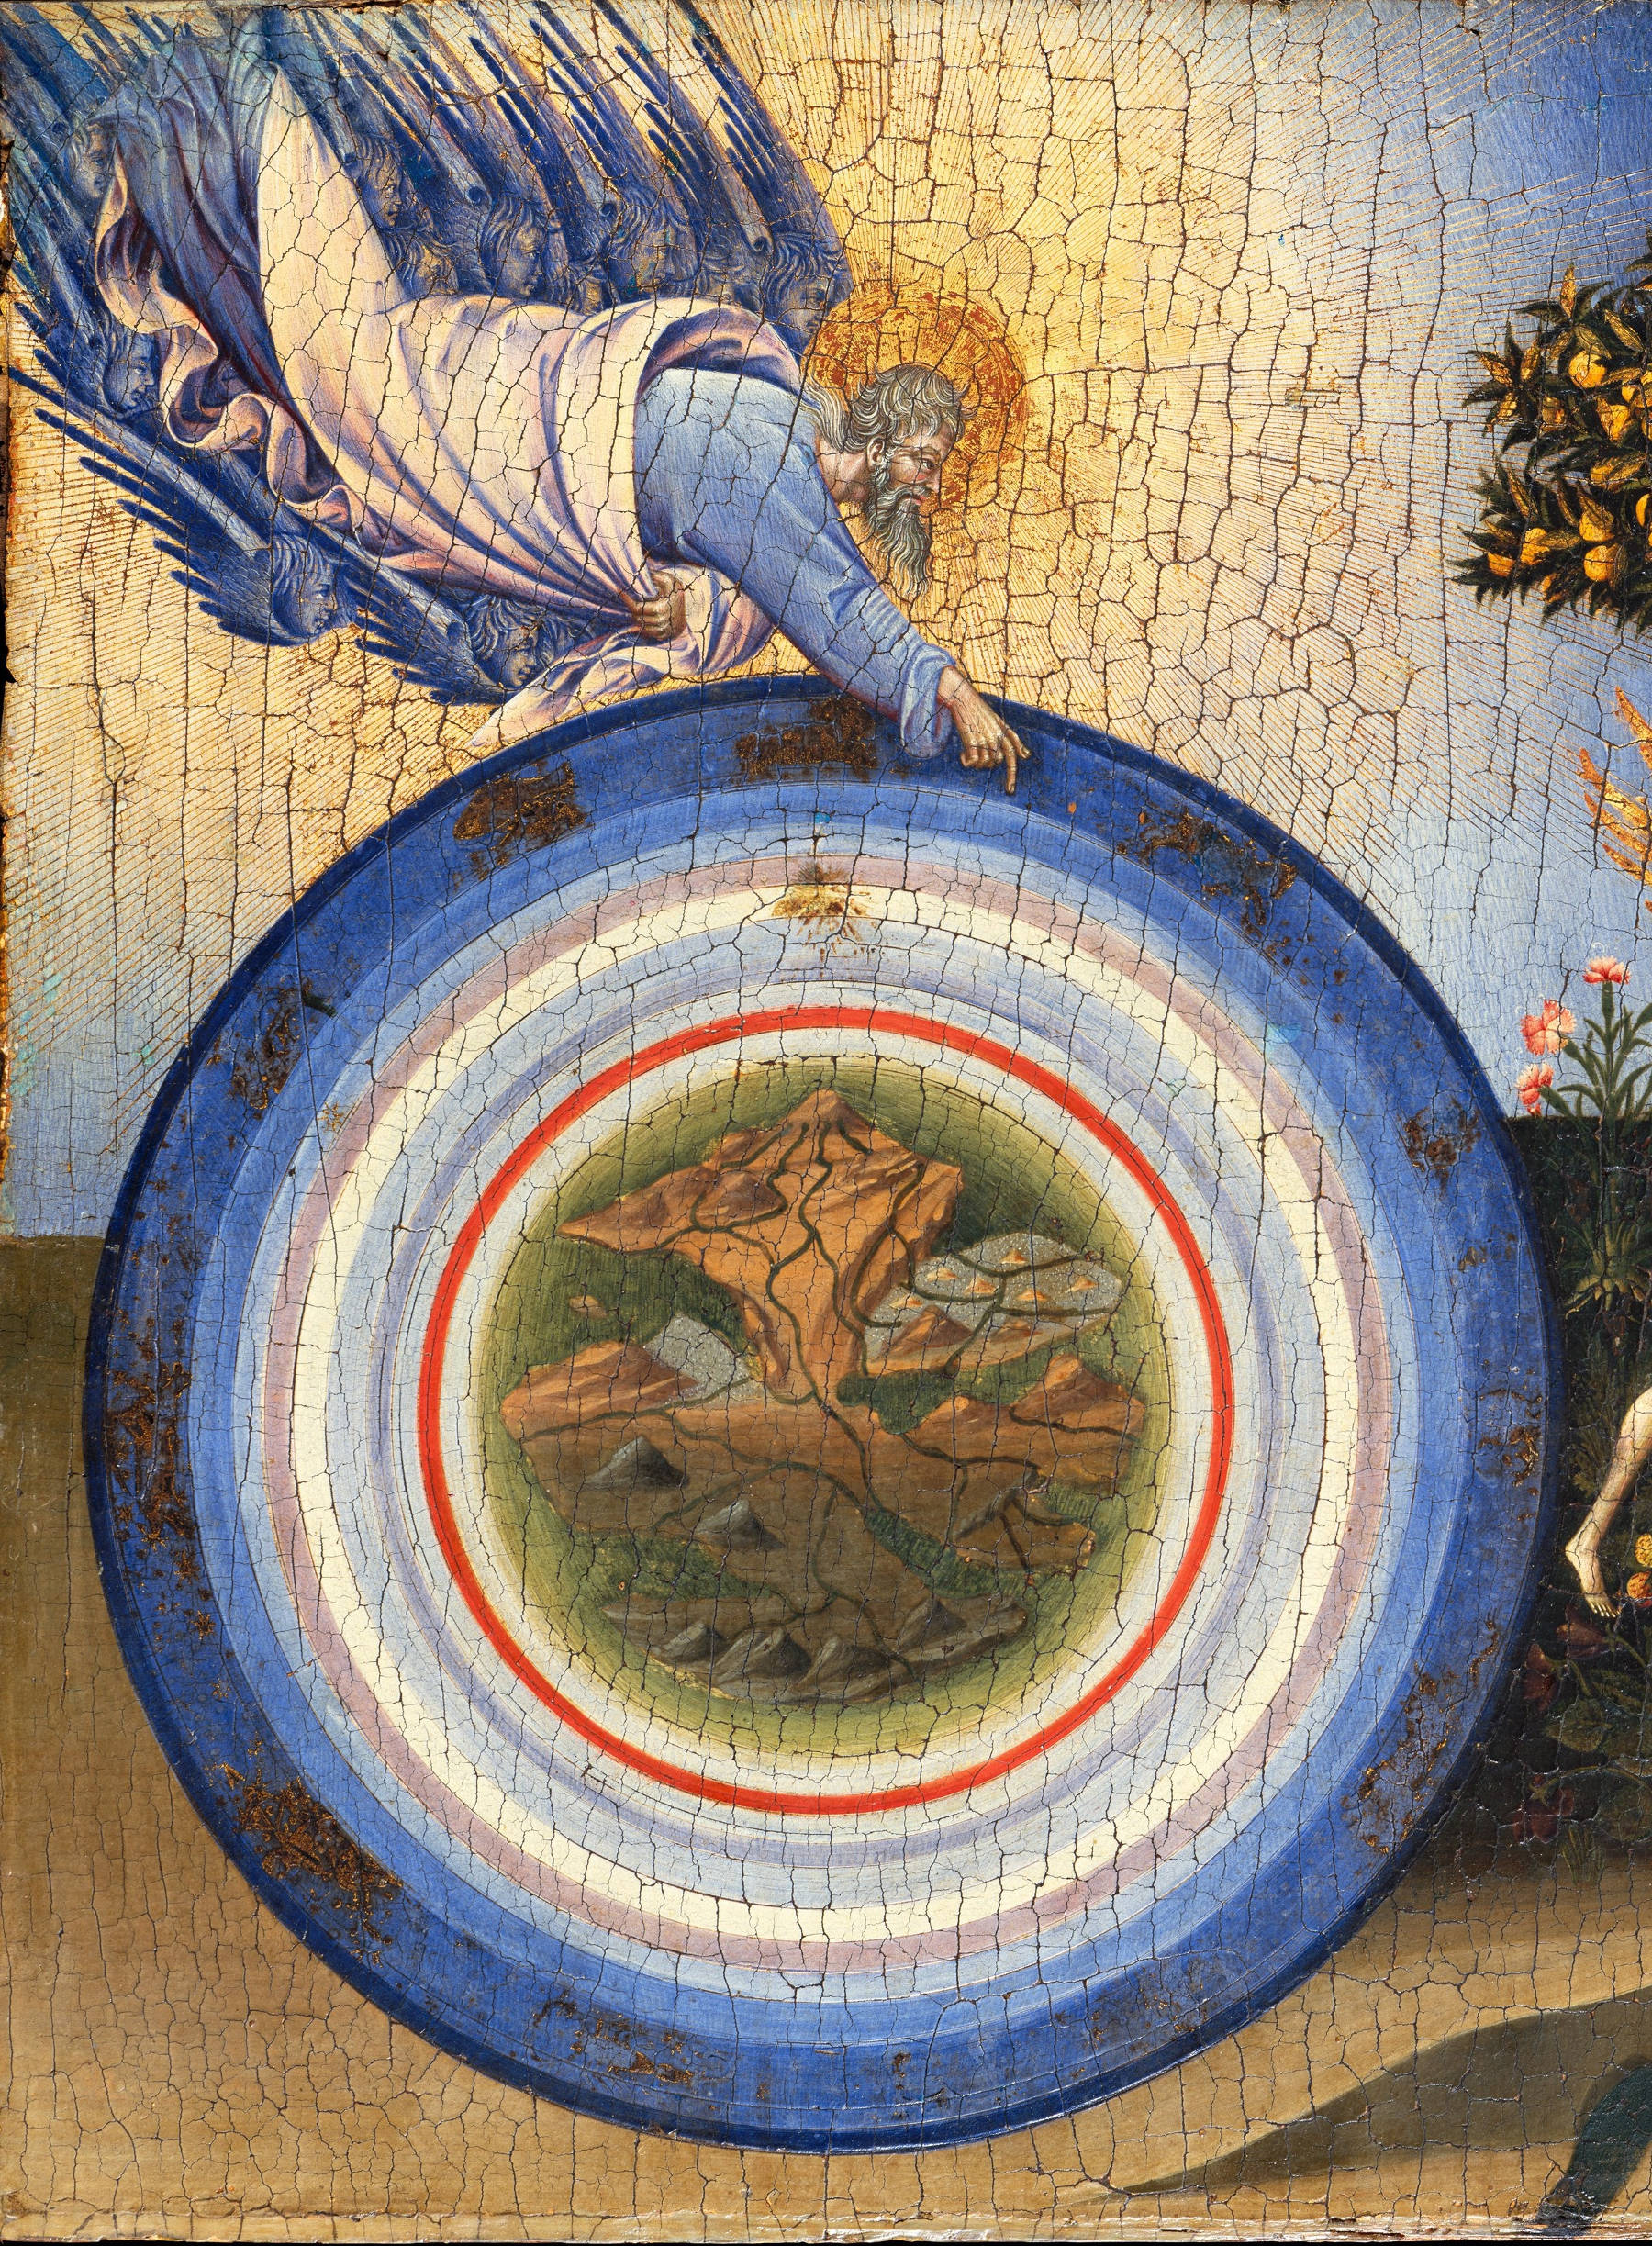
\includegraphics[width=\linewidth,trim={0 1cm 0 2cm},clip]{img/Giovanni_di_Paolo_-_Creation.jpg}
        \column{.5\textwidth}
            \centering
            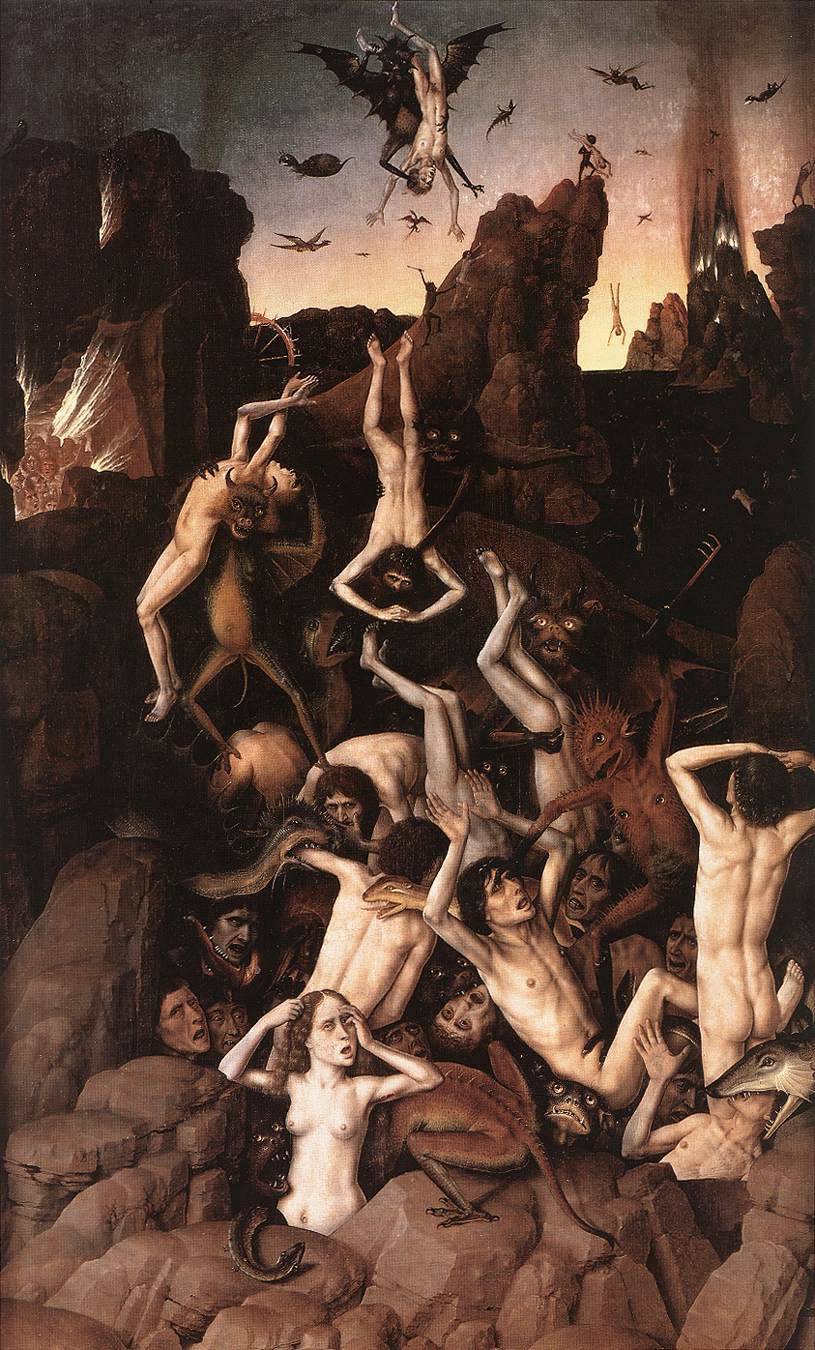
\includegraphics[width=\linewidth,trim={0 1cm 0 1.7cm},clip]{img/Dirk_Bouts_-_Hell.jpg}
    \end{columns}
\end{frame}

\subsection{Distro}

\begin{frame}{Fundamentals}
    \begin{itemize}
        \item what is Linux
        \item what is distro
        \item what is Linux distro
        \item what is version
        \item what is semantic version
        \item what is Linux distro version
        \item what is Linux distro package metadata
    \end{itemize}
\end{frame}

\begin{frame}{What is Yocto?}
    \begin{block}{}
        Yocto allows you to build a distro on your own.
    \end{block}
    \begin{center}
        
\includegraphics[width=0.5\linewidth]{img/Yocto_Logo.png}
    \end{center}
    \begin{block}{}
        \url{https://www.yoctoproject.org/}
    \end{block}
\end{frame}

\subsection{ECL}

\begin{frame}{The world of ecl}
    \begin{itemize}
        \item what is ecl
        \item what is lfs
        \item what is relation between distro version and ecl
    \end{itemize}
\end{frame}

\section{Artifacts}

\begin{frame}{Artifacts: sdk, package and index}
    \centering
    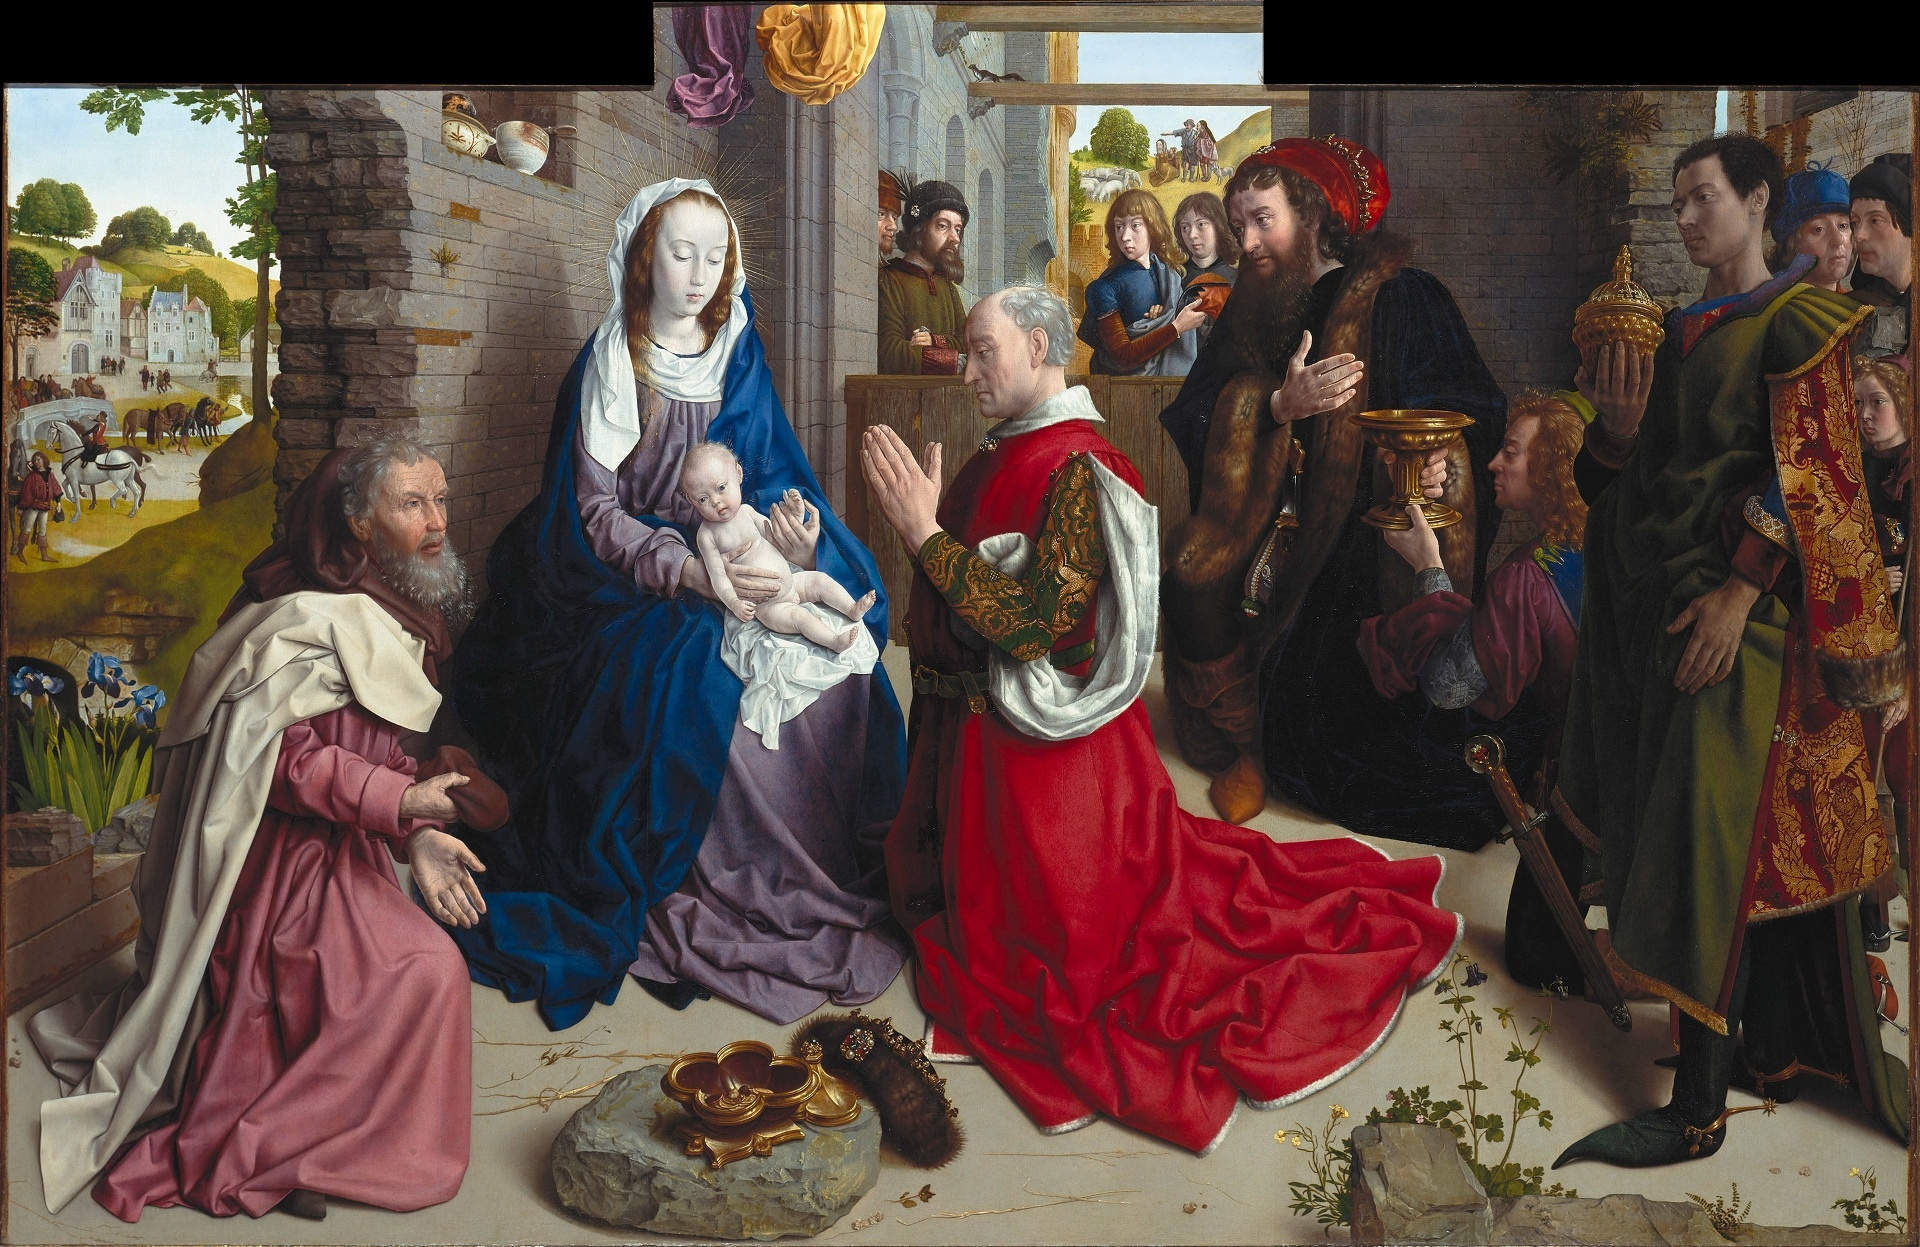
\includegraphics[width=\linewidth]{img/Hugo_van_der_Goes_-_The_Adoration_of_the_Kings.jpg}
\end{frame}

\subsection{SDK}

\begin{frame}{What is SDK?}
    \begin{block}{}
        An \textbf{SDK} is a toolchain and sysroot.
    \end{block}
    \begin{block}{}
        It has essentials needed to develop for particular platform.
    \end{block}
    \begin{block}{}
        It should work on any machine developer may use.
    \end{block}
    \begin{block}{}
        It is self contained.
    \end{block}
\end{frame}

\begin{frame}[fragile]{SDK installs}
\begin{block}{}
SDK comes in form of installable shell script: shar
(shell archive).
\end{block}
\begin{lstlisting}[style=Console]
$ ./***-toolchain-***.sh
Enter target directory for SDK (default: /opt/***/1.6.1): sdk
You are about to install the SDK to "/***/sdk". Proceed[Y/n]?
Extracting SDK...done
Setting it up...done
SDK has been successfully set up and is ready to be used.
\end{lstlisting}
\end{frame}

\begin{frame}[fragile]{SDK has a directory structure}
\begin{block}{}
\begin{itemize}
\item{setup script}
\item{target sysroot}
\item{toolchain sysroot}
\end{itemize}
\end{block}
\begin{lstlisting}[style=TinyConsole]
sdk
|-- environment-setup-core2-64-nokia-linux
|-- site-config-core2-64-nokia-linux
|-- sysroots
|   |-- core2-64-nokia-linux
|   |   |-- etc
|   |   |-- lib64
|   |   |-- usr
|   |   \-- var
|   \-- i686-nsnsdk-linux
|       |-- bin
|       |-- etc
|       |-- lib
|       |-- usr
|       |-- var
|       \-- x86_64-pc-linux-gnu
\-- version-core2-64-nokia-linux
\end{lstlisting}
\end{frame}

\begin{frame}[fragile, t]{SDK has environment script}
    \begin{block}{}
        Source it to enter SDK environment. \\
        \begin{columns}
            \centering
            \begin{column}{.9\textwidth}
\begin{lstlisting}[style=TinyConsole]
source sdk/environment-setup-core2-64-nokia-linux
\end{lstlisting}
            \end{column}
        \end{columns}
    \end{block}
    \begin{block}{}
        Sets path, auxiliary and program specific variables:
        \begin{itemize}
            \scriptsize
            \item<1->{to know location of sysroots}
            \item<2->{to use \verb|[archprefix]-gcc|, \verb|cmake|, \verb|opkg|}
            \item<3->{\verb|CC|, \verb|CXX|, \verb|LD| for build tool to detect}
            \item<4->{for \verb|pkg-config|, \verb|opkg|, \verb|python| to use sdk}
            \item<5->{libdir and dynlinker to execute binaries}
        \end{itemize}
    \end{block}
    \begin{onlyenv}<1>
\begin{lstlisting}[style=TinyConsole]
export SDKTARGETSYSROOT=/***/sdk/sysroots/core2-64-nokia-linux
export OECORE_NATIVE_SYSROOT="/***/sdk/sysroots/i686-nsnsdk-linux"
\end{lstlisting}
    \end{onlyenv}
    \begin{onlyenv}<2>
\begin{lstlisting}[style=TinyConsole]
export PATH=/***/sdk/sysroots/i686-nsnsdk-linux/usr/bin: \
            /***/sdk/sysroots/i686-nsnsdk-linux/usr/bin/x86_64-nokia-linux: \
            $PATH
\end{lstlisting}
    \end{onlyenv}
    \begin{onlyenv}<3>
\begin{lstlisting}[style=TinyConsole]
export CC="x86_64-pc-linux-gnu-gcc -m64 --sysroot=$SDKTARGETSYSROOT"
export CXX="x86_64-pc-linux-gnu-g++ -m64 --sysroot=$SDKTARGETSYSROOT"
export CPP="x86_64-pc-linux-gnu-gcc -E -m64 --sysroot=$SDKTARGETSYSROOT"
export LD="x86_64-pc-linux-gnu-ld --sysroot=$SDKTARGETSYSROOT"
\end{lstlisting}
    \end{onlyenv}
    \begin{onlyenv}<4>
\begin{lstlisting}[style=TinyConsole]
export PKG_CONFIG_SYSROOT_DIR=$SDKTARGETSYSROOT
export PKG_CONFIG_PATH=$SDKTARGETSYSROOT/usr/lib64/pkgconfig
export OFFLINE_ROOT=$SDKTARGETSYSROOT
export PYTHONPATH=$OECORE_NATIVE_SYSROOT/usr/lib/python2.7/site-packages:$PYTHONPATH
\end{lstlisting}
    \end{onlyenv}
    \begin{onlyenv}<5>
\begin{lstlisting}[style=TinyConsole]
export SYSROOT_LIB_DIR=$SDKTARGETSYSROOT/usr/lib64:$SDKTARGETSYSROOT/lib64
export SYSROOT_DYN_LINKER=$SDKTARGETSYSROOT/lib64/ld-linux-x86-64.so.2
\end{lstlisting}
    \end{onlyenv}
\end{frame}

\begin{frame}[fragile]{SDK toolchain has compilers and tools}
\begin{lstlisting}[style=Console]
i686-nsnsdk-linux
|-- bin
|   |-- x86_64-pc-linux-gnu-g++
|   |-- x86_64-pc-linux-gnu-gcc
|   |-- x86_64-pc-linux-gnu-ld
|   |-- x86_64-pc-linux-gnu-nm
|   |-- x86_64-pc-linux-gnu-readelf
|   |-- x86_64-pc-linux-gnu-size
|   |-- x86_64-pc-linux-gnu-strings
|   \-- x86_64-pc-linux-gnu-strip
\-- usr
    \-- bin
        |-- cmake
        |-- opkg -> opkg-cl
        |-- opkg-cl
        |-- pkg-config
        |-- prophyc
        \-- protoc
\end{lstlisting}
\end{frame}

\begin{frame}[fragile, t]{SDK sysroot holds target-related stuff}
    \begin{block}{}
        \begin{itemize}
            \item<1->{executables \& scripts}
            \item<2->{libraries \& headers \& pc files}
            \item<3->{configuration}
            \item<4->{data}
        \end{itemize}
    \end{block}
    \begin{onlyenv}<1>
\begin{lstlisting}[style=Console]
usr
\-- bin
    \-- CCSDaemonExe
\end{lstlisting}
    \end{onlyenv}
    \begin{onlyenv}<2>
\begin{lstlisting}[style=Console]
usr
|-- include
|   \-- boost
|       \-- chrono
|           \-- chrono.hpp
\-- lib64
    |-- pkgconfig
    |   \-- prophy.pc
    |-- libboost_chrono.so -> libboost_chrono.so.1.59.0
    \-- libboost_chrono.so.1.59.0
\end{lstlisting}
    \end{onlyenv}
    \begin{onlyenv}<3>
\begin{lstlisting}[style=Console]
etc
\-- opkg
    \-- opkg.conf
\end{lstlisting}
    \end{onlyenv}
    \begin{onlyenv}<4>
\begin{lstlisting}[style=Console]
usr
\-- share
    \-- bpf
        \-- bpf.xml
\end{lstlisting}
    \end{onlyenv}
\end{frame}

\begin{frame}{SDK sysroot is filled bottom-up}
    \begin{block}{}
        \begin{itemize}
            \item{may be empty after sdk deployment}
            \item{will be filled according to dependencies}
            \begin{itemize}
                \item{by package manager \& server}
                \item{by manual package installation}
                \item{by manual build \& installation from source}
            \end{itemize}
        \end{itemize}
    \end{block}
\end{frame}

\subsection{Package}

\begin{frame}[fragile]{Package has format}
    \begin{block}{}
        Packages fulfil a certain format, which package manager can understand.
    \end{block}
    \begin{block}{}
        Opkg requires \verb|.ipk| packages, format similar to \verb|.deb|.
    \end{block}
\end{frame}

\begin{frame}[fragile]{Package has name}
    \begin{block}{}
        There are 3 sections separated by underscores
        \begin{itemize}
            \item<2->{name \only<3->{and purpose}}
            \item<4->{version}
            \item<5->{architecture}
        \end{itemize}
    \end{block}
\begin{onlyenv}<1>\begin{lstlisting}[style=Console]
liblim-dev_0~FL00-LIM-0001-07-2898-r0_core2-64.ipk
\end{lstlisting}\end{onlyenv}
\begin{onlyenv}<2>\begin{lstlisting}[style=Console]
lib@@@lim@@@-dev_0~FL00-LIM-0001-07-2898-r0_core2-64.ipk
\end{lstlisting}\end{onlyenv}
\begin{onlyenv}<3>\begin{lstlisting}[style=Console]
@@@liblim-dev@@@_0~FL00-LIM-0001-07-2898-r0_core2-64.ipk
\end{lstlisting}\end{onlyenv}
\begin{onlyenv}<4>\begin{lstlisting}[style=Console]
liblim-dev_@@@0~FL00-LIM-0001-07-2898-r0@@@_core2-64.ipk
\end{lstlisting}\end{onlyenv}
\begin{onlyenv}<5>\begin{lstlisting}[style=Console]
liblim-dev_0~FL00-LIM-0001-07-2898-r0_@@@core2-64@@@.ipk
\end{lstlisting}\end{onlyenv}
\end{frame}

\begin{frame}[fragile]{Package has purpose}
    \begin{block}{}
        Usually single project is partitioned to several packages.
        Each package serves a different purpose.
    \end{block}
    \begin{itemize}
        \item{
            dynamic library \hfill to run
\begin{lstlisting}[style=Console]
liblim1_0~FL00-LIM-0001-07-2898-r0_core2-64.ipk
\end{lstlisting}
        }
        \item{
            debug symbols and source code \hfill to debug
\begin{lstlisting}[style=Console]
liblim-dbg_0~FL00-LIM-0001-07-2898-r0_core2-64.ipk
\end{lstlisting}
        }
        \item{
            headers, library link, \verb|.pc| file \hfill to link against
\begin{lstlisting}[style=Console]
liblim-dev_0~FL00-LIM-0001-07-2898-r0_core2-64.ipk
\end{lstlisting}
        }
        \item{
            static library \hfill to link against all symbols
\begin{lstlisting}[style=Console]
liblim-staticdev_0~FL00-LIM-0001-07-2898-r0_core2-64.ipk
\end{lstlisting}
        }
    \end{itemize}
\end{frame}

\begin{frame}[fragile]{Package has directory layout}
    \begin{block}{}
        Package is a compressed archive with directory structure
        \begin{itemize}
            \item{piece of sysroot to install}
            \item{metadata}
        \end{itemize}
    \end{block}
\begin{lstlisting}[style=Console]
liblim-dev_0~FL00-LIM-0001-07-2898-r0_core2-64.ipk
|-- CONTENTS
|   \-- usr
|       |-- include
|       |   \-- lim
|       |       \-- ...
|       \-- lib64
|           |-- liblim.so -> liblim.so.1
|           \-- pkgconfig
|               \-- lim.pc
|-- DEBIAN
|   \-- control
|-- INFO
\-- INSTALL
\end{lstlisting}
\end{frame}

\begin{frame}[fragile]{Package has metadata}
    \begin{block}{}
        File \verb|DEBIAN/control| contains package metadata.
    \end{block}
\begin{lstlisting}[style=Console]
@@@Package: liblim-dev@@@
@@@Version: 0~FL00-LIM-0001-07-2898-r0@@@
Description: *****
Section: devel
Priority: optional
Maintainer: *****
License: CLOSED
@@@Architecture: core2-64@@@
OE: lim
@@@Depends: liblim1 (= 0~FL00-LIM-0001-07-2898-r0)@@@
Recommends: *****
Source: *****
\end{lstlisting}
\end{frame}

\begin{frame}[fragile]{Package has dependencies}
    \begin{block}{}
        Packages usually depend on others.
    \end{block}
\begin{lstlisting}[style=Console]
Package: zeya
...
Depends: python (>= 2.7.1-0ubuntu2), vorbis-tools,
    python-simplejson, python-tagpy
Recommends: mpg123, flac, faad
\end{lstlisting}
    \begin{block}{}
        This allows package manager to fetch dependencies
        automatically. It helps to keep system integrity
        during upgrades or removals.
    \end{block}
\end{frame}

\begin{frame}[fragile]{Package has project information}
    \begin{block}{}
        Package metadata alone can point to
        rich source of project related information.
    \end{block}
\begin{lstlisting}[style=Console]
Package: opera
...
Maintainer: Opera Packaging Team <packager@opera.com>
Bugs: https://bugs.opera.com/wizard/
Homepage: http://www.opera.com/browser/
\end{lstlisting}
    \begin{block}{}
        This data is easy to keep up to date since
        packages update constantly.
    \end{block}
\end{frame}

\begin{frame}[fragile]{Package can have documentation}
    \begin{block}{}
        \renewcommand{\arraystretch}{1.5}
        \begin{tabular}{l l}
            readme & \small\verb|/usr/share/doc/valgrind/README| \\
            changelog & \small\verb|/usr/share/doc/valgrind/NEWS.Debian.gz| \\
            authors & \small\verb|/usr/share/doc/valgrind/AUTHORS| \\
            man pages & \small\verb|/usr/share/man/man1/valgrind.1.gz| \\
            html docs & \small\verb|/usr/share/doc/valgrind/html/index.html| \\
        \end{tabular}
    \end{block}
\end{frame}

\begin{frame}[fragile]{Package can be arch-agnostic}
    \begin{block}{}
        Packages which contain no machine-specific files,
        e.g. only scripts, data or headers, can have architecture \verb|all|.
    \end{block}
    \begin{block}{}
        Such packages are reused
        between different architectures of a distro.
    \end{block}
\begin{lstlisting}[style=Console]
bpf_42160-r0_all.ipk
\end{lstlisting}
\begin{lstlisting}[style=Console]
.
`-- CONTENTS
    `-- usr
        `-- share
            `-- bpf
                `-- bpf.xml
\end{lstlisting}
\end{frame}

\subsection{Index}

\begin{frame}[fragile]{Index lists packages}
    \begin{block}{}
        Index file contains information about distribution.
        It's a text file with concatenated package metadata
        (same key-value pairs as in DEBIAN/control).
    \end{block}
    \begin{block}{}
        It's named \verb|Packages| or - if compressed - \verb|Packages.gz|.
    \end{block}
\begin{lstlisting}[style=Console]
Package: project1
Version: 1.2.0
Recommends: project2
...

Package: project2
Version: 0.3.0
Depends: project3 (= 1.1.0), project4 (>= 2.3.0)
...

... ... ...
\end{lstlisting}
\end{frame}

\begin{frame}[fragile]{Index is compressed}
Index file is usually stored and downloaded compressed.
It's large and text - compresses well.
\begin{lstlisting}[style=Console]
38195 Oct 27 10:27 Packages
 5212 Oct 27 10:27 Packages.gz
\end{lstlisting}
\end{frame}

\begin{frame}[fragile, t]{Index family is a distro}
    \begin{block}{}
        Index file groups packages belonging to specific:
        \begin{itemize}
            \item<1-> architecture
            \item<2-> version
            \item<3-> release
        \end{itemize}
    \end{block}
\begin{onlyenv}<1>\begin{lstlisting}[style=TinyConsole]
51971
|-- all
|   `-- @@@Packages.gz@@@
|-- core2-64
|   `-- @@@Packages.gz@@@
|-- cortexa15hf-vfp
|   `-- @@@Packages.gz@@@
|-- i586
|   `-- @@@Packages.gz@@@
|-- mips64-nf
|   `-- @@@Packages.gz@@@
`-- ppce500
    `-- @@@Packages.gz@@@
\end{lstlisting}\end{onlyenv}
\begin{onlyenv}<2>\begin{lstlisting}[style=TinyConsole]
ECL
|-- @@@51955@@@
|-- @@@51962@@@
|-- @@@51965@@@
|-- @@@51971@@@
`-- @@@51988@@@
\end{lstlisting}\end{onlyenv}
\begin{onlyenv}<3>\begin{lstlisting}[style=TinyConsole]
.
|-- BTS_SCM_LTE_ECL
|   `-- trunk
|       `-- ECL_SACK_BASE
|           `-- @@@ECL@@@
`-- BTS_SCM_OAM_LTE_ECL
    |-- branches
    |   `-- maintenance
    |       `-- xL15A
    |           `-- ECL_OAM
    |               `-- @@@ECL@@@
    `-- trunk
        `-- ECL_OAM
            `-- @@@ECL@@@
\end{lstlisting}\end{onlyenv}
\end{frame}

\section{Roles}

\begin{frame}{Roles: developer and maintainer}
    \centering
    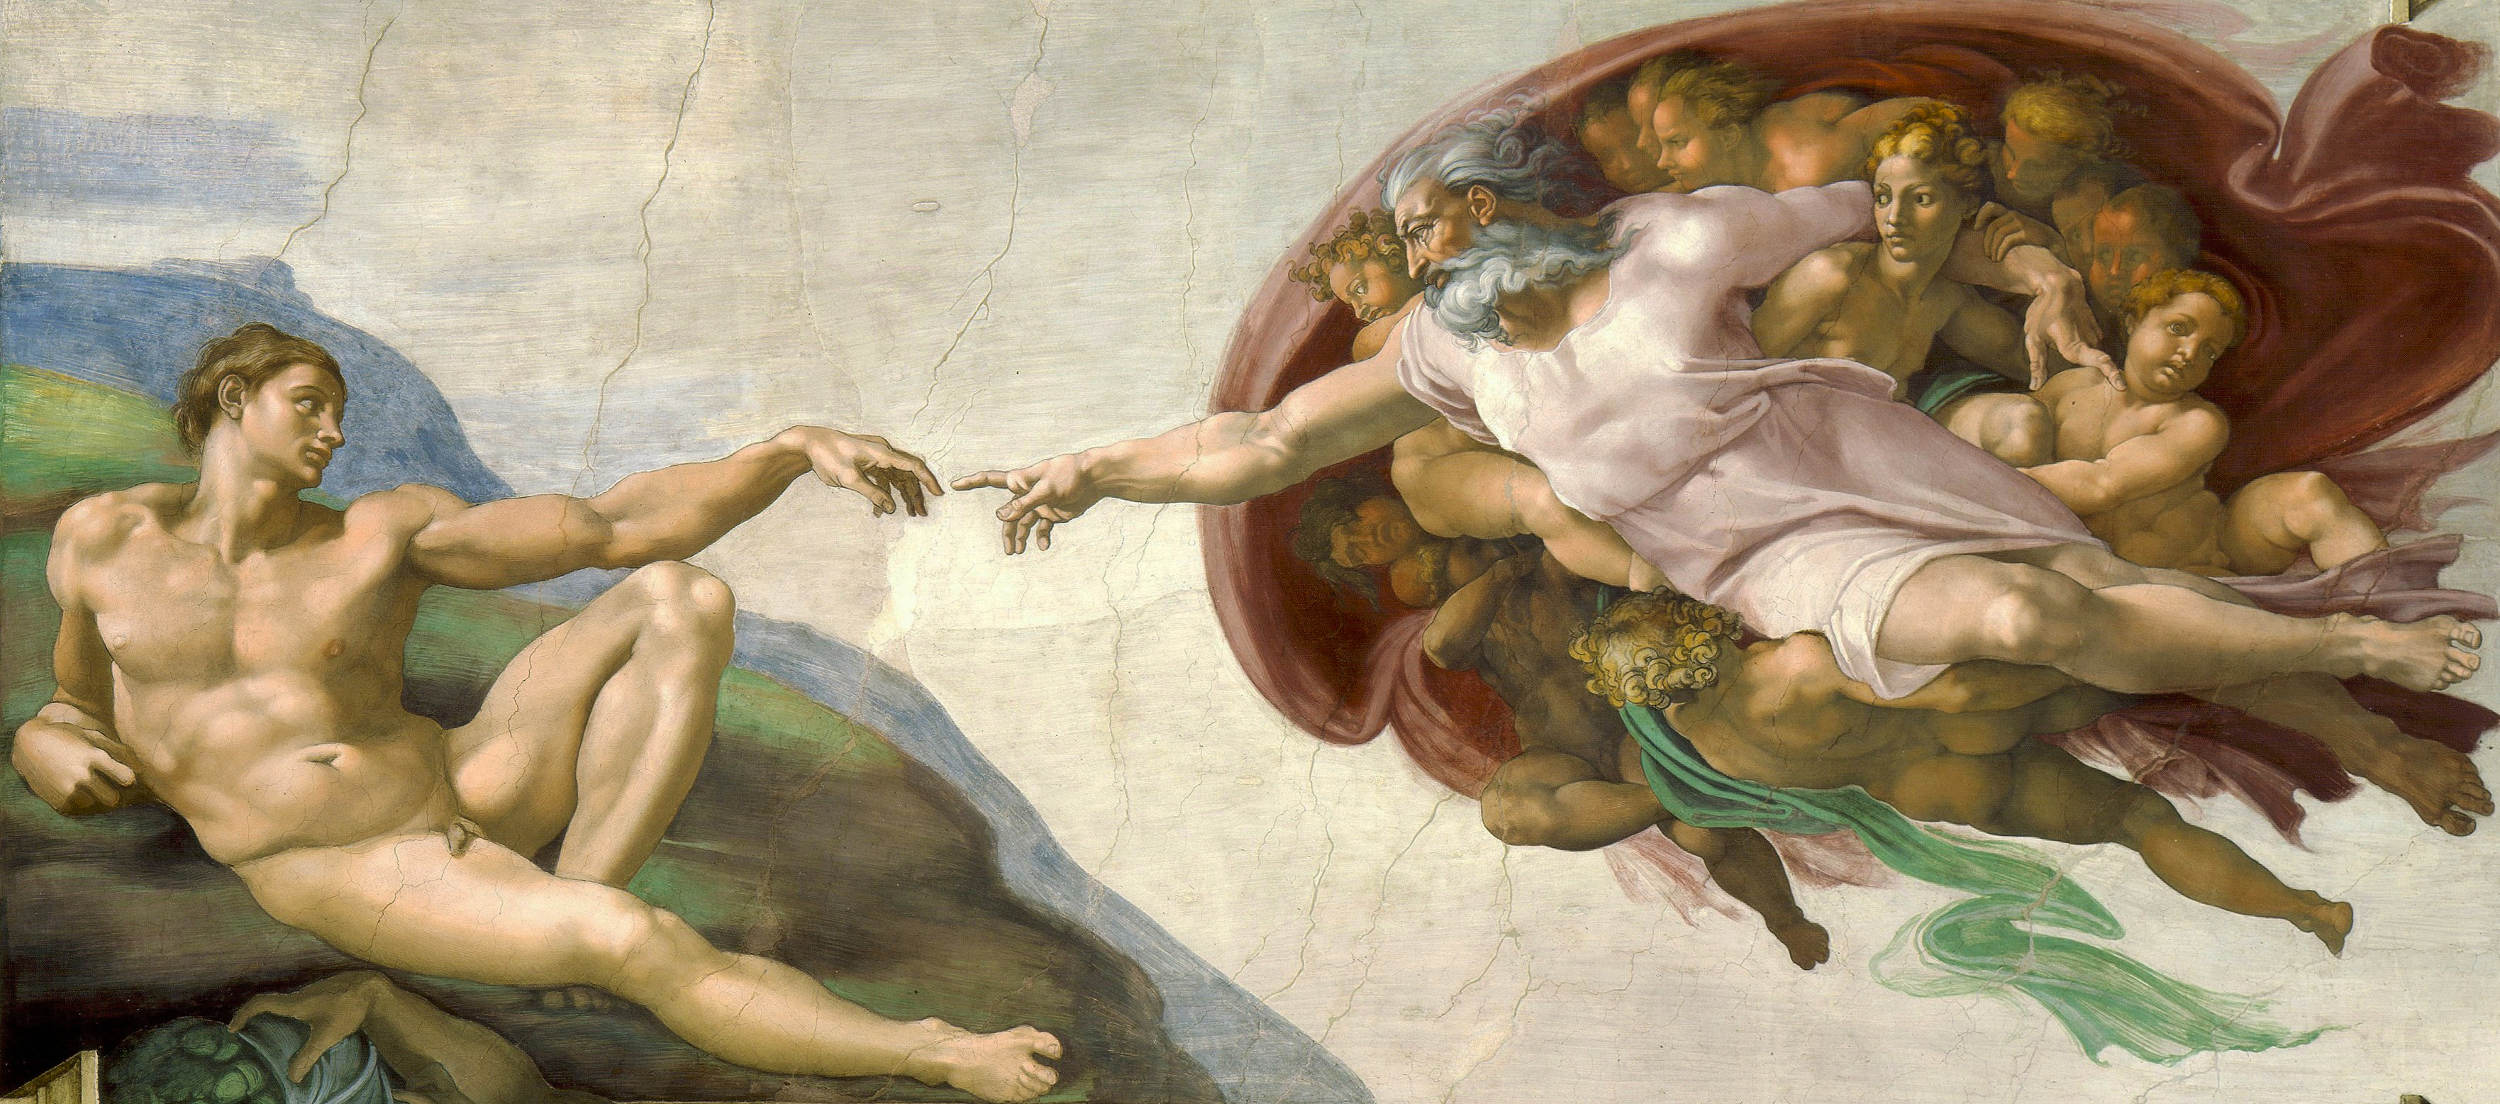
\includegraphics[width=\linewidth]{img/Michelangelo_-_The_Creation_of_Adam.jpg}
\end{frame}

\subsection{Developer}

\begin{frame}[fragile]{Developer uses sdk}
    \begin{block}{}
        Developer downloads sdk, fills it by:
        \begin{itemize}
            \item installation by package manager
            \item installation by \verb|.ipk| package
            \item installation by building sources
        \end{itemize}
        and compiles/tests his code.
    \end{block}
    \begin{block}{}
        \color{green!60!black}
        Developer may play with sdk contents and change, mix, hack, corrupt them.
        Recreating sdk with dependencies is cheap and takes a minute.
    \end{block}
\end{frame}

\begin{frame}[fragile]{Developer respects rules}
    \begin{block}{This saves the day for maintainers}
        Conform to linux directory structure.
        Install relevant things in \verb|include|, \verb|bin|,
        \verb|lib[64]|, \verb|share|, \verb|.pc|.
    \end{block}
    \begin{block}{This saves the day for your users}
        Be very strict about public API.
        Separate it clearly from internal logic.
        Keep source, binary and functional compatibility in check.
    \end{block}
    \begin{block}{}
        \color{red!60!black}
        Developer doesn't use bitbake. \\
        Developer doesn't have to write recipes.
    \end{block}
\end{frame}

\begin{frame}{Let's build \color{blue}{(example)}}
    Once upon a time there was a project. \\
    Let's build and test it:
    \begin{multicols}{2}
        \begin{enumerate}
            \item Download proper sdk.
            \item Install sdk.
            \item Source sdk environment.
            \item Set proper distro.
            \item Download index.
            \item Download packages.
            \item Configure.
            \item Build unit tests.
            \item Run unit tests.
            \item Build binaries.
            \item Install binaries.
            \item Run functional tests.
        \end{enumerate}
    \end{multicols}
\end{frame}

\begin{frame}[fragile]{Let's CI \color{blue}{(example)}}
    Once upon a time there was a different project. \\
    Let's inspect its CI scripts:
    \vspace{\baselineskip}
    \begin{enumerate}
        \item Build commands in \verb|Makefile.ci|.
        \item Buildbot \verb|master.cfg|.
        \item Buildbot web api.
        \item Build machines.
    \end{enumerate}
\end{frame}

\subsection{Maintainer}

\begin{frame}{Maintainer produces sdk \& packages}
    \begin{block}{}
        Maintainer maintains:
        \begin{itemize}
            \item{in-house bitbake layer repositories}
            \item{building machines}
            \item{sdk \& package file servers}
        \end{itemize}
    \end{block}
    \begin{block}{}
        \color{red!60!black}
        Maintainer doesn't release project versions. \\
        Maintainer doesn't care about project CIs.
    \end{block}
\end{frame}

\begin{frame}[fragile]{Maintainer upgrades distro}
    \begin{block}{}
        Distro upgrades:
        \begin{itemize}
            \item{when project releases new version}
            \item{when dependencies change}
            \item{when new project gets added}
        \end{itemize}
    \end{block}
    \begin{block}{}
        Maintainer commits changes to recipes (usually renames).
        This rebuilds and uploads new packages to file server.
    \end{block}
    \begin{block}{}
        \color{green!60!black}
        Maintainer can change version of a project
        and build image without influencing developers. \\
        Should integration prove troublesome, he can ask specific
        projects to provide patches or adapted versions.
    \end{block}
\end{frame}

\begin{frame}[fragile]{Maintainer adds products}
    \begin{block}{}
        Each time when new board or processor architecture
        appears maintainer adds a product dir for it.
    \end{block}
    \begin{block}{}
        \color{green!60!black}
        Effort to introduce new product is small, since:
        \begin{itemize}
            \color{green!60!black}
            \item{cpu architecture config (gcc target, tune)}
            \item{kernel config, drivers, board support package}
            \item{user space recipes}
        \end{itemize}
        are largely orthogonal.
    \end{block}
\end{frame}

\begin{frame}[fragile]{Let's peek at recipe repository \color{blue}{(example)}}
    Bitbake recipes are held in repository.
    \vspace{\baselineskip}
    \begin{enumerate}
        \item{It bases on \verb|poky|: yocto reference distro.}
        \item{It has subdirectories for products.}
        \item{It has subdirectories for layers.}
        \item{It has branches for releases.}
    \end{enumerate}
\end{frame}

\begin{frame}[fragile]{Let's peek at continuous package builder \color{blue}{(example)}}
    When ecl changes, distro upgrades.
    \vspace{\baselineskip}
    \begin{enumerate}
        \item{Ecl watcher detects the change.}
        \item{Change gets committed as recipes renames.}
        \item{Yocto CI reacts building and uploading packages.}
    \end{enumerate}
\end{frame}

\begin{frame}[fragile]{Let's peek at buildbot webapi \color{blue}{(example)}}
    Machines building packages may fail.
    \vspace{\baselineskip}
    \begin{enumerate}
        \item{Packages must be built constantly and quickly.}
        \item{Problems need to be spotted fast.}
        \item{Machines need to be powerful or numerous enough.}
    \end{enumerate}
\end{frame}

\begin{frame}[fragile]{Let's peek at file server \color{blue}{(example)}}
    Package file server is constantly used by developers.
    \vspace{\baselineskip}
    \begin{enumerate}
        \item{Capacious: packages may take a lot of disk space.}
        \item{Secure: recent packages need to be held intact.}
        \item{Fast: lots of downloads.}
        \item{Accessible: users may need access at any time.}
    \end{enumerate}
\end{frame}

\appendix

\section{\appendixname}

\subsection{Examples reference}

\begin{frame}
    \setbeamersize{description width=-\labelsep}
    \begin{description}
        \item[Build project] \hfill \\
            \begin{dummyenv}
                \color{blue}\scriptsize
                \url{https://en.wikibooks.org} \\
                \url{https://en.wikibooks.org} \\
                \url{https://en.wikibooks.org/wiki/LaTeX/List_Structures} \\
            \end{dummyenv}
        \item[CI project] \hfill \\
            \begin{dummyenv}
                \color{blue}\scriptsize
                \url{https://en.wikibooks.org} \\
                \url{https://en.wikibooks.org} \\
                \url{https://en.wikibooks.org/wiki/LaTeX/List_Structures} \\
            \end{dummyenv}
        \item[Maintainer stuff] \hfill \\
            \begin{dummyenv}
                \color{blue}\scriptsize
                \url{https://en.wikibooks.org} \\
                \url{https://en.wikibooks.org} \\
                \url{https://en.wikibooks.org/wiki/LaTeX/List_Structures} \\
            \end{dummyenv}
    \end{description}
\end{frame}

\subsection{Questions}

\begin{frame}
    \begin{center}
        \Huge Questions
    \end{center}
\end{frame}

\end{document}